\chapter{Improving Channel Estimation}\label{ch:channel_estimation}

Estimating the channel in the wireless transmission is essential and paramount to achieving effective communication. The estimation of the channel effectively improves the recovery of the received bits by \emph{equalizing} the imposed channel conditions, as presented in chapter \ref{ch:mlbasics} discussing the use of adaptive filters. In simple terms, the operation of equalization implies the removal of channel effects such that the original bits can be recovered with a reduced amount of errors. However, to do so, channel estimation is required, i.e. computing and approximating the channel matrix $H$ \cite{Cho2010MIMO-OFDMMATLAB}. Achieving accurate channel estimations is directly translatable to improved transmission data rates, and enables the practicalities of the essential \gls{mimo} solutions. This chapter will present a brief overview of existing channel estimation techniques and discuss the application of Deep Learning herein. 

A comprehensive survey of existing methods can be found in  \cite{Cho2010MIMO-OFDMMATLAB, Liu2014ChannelOFDM} and references herein. Two typical families of channel estimation methods are commonly presented throughout the literature and are termed \gls{dde} and \gls{pe}. The former is also known as blind channel estimation where the channel statistics are derived from the demodulated data. The latter (and the methods related) is the primary scope of this chapter. \gls{pe} utilize known reference signals, also known as pilot signals, to calculate the channel conditions and the matrix $H$.


\section{Pilot-based channel estimation techniques}\label{sec:channel_estimators}
The pilot signals, e.g. pilot symbols, is used to estimate the channel conditions by using a preamble of symbols that are known to both the transmitter and the receiver. Placing the pilot symbols in both time and frequency enable the necessary information and thus statistics of the channel to be captured. On top of the pilot placement, the number of required pilot symbols are minimized by employing an estimation strategy. The estimation strategy involves estimating the entirety of the channel response using only a few samples and therefor decreasing the transmission overhead associated with the pilot symbols. These pilot symbols, while they are essential, occupy bandwidth that may otherwise be used for valuable data transmission.

We denote a communication system by the following (simplified) operation in frequency.


\begin{equation}
    Y = X \cdot H + \epsilon
\end{equation}

Where $Y$ is the received signal, $X$ is the transmitted signal, $H$ are the channel coefficients and $\epsilon$ is measurement noise. The task is to estimate the channel matrix $H$ using pilot signals. If a full knowledge of Y, i.e. for all frequency components can be obtained, a perfect estimation of the channel $H$ can be achieved, limited by the interval of the pilot signals. However, in practice, it would mean that no components can be used for actual data transmission. Thus the objective is to minimize the number of pilot symbols and maximize the knowledge of the matrix $H$. A channel estimator function, $Z(\cdot)$ is used for this purpose, obtaining an estimation $\hat{H}$ of the matrix $H$ by applying techniques to a sparse and noisy amount of received pilot signals $Y_p$. 

\begin{equation}
    \hat{H} = Z(Y_p)
\end{equation}

By knowing the location of the received pilot signals, in both time and frequency, techniques can be applied to estimate the matrix $H$. Improving the performance of the channel estimator is directly translatable to optimizing the transmission. The result is more accurate demodulation, equalization and decoding of the received signal with fewer errors.



\subsection{Traditional methods}

Various methods exist for obtaining the function $Z(\cdot)$ \cite{Oyerinde2012ReviewSystems}. One example is the linear estimator denoted by the use of \gls{ls} estimation (essentially the adaptive filter mentioned in Chapter \ref{ch:mlbasics}). \acrlong{ls} channel estimators are straightforward and simple to implement as opposed to the \gls{mmse} channel estimation that requires statistical knowledge of the channel but can offer improved performance. Both are essentially linear estimators resulting in a linear interpolation between the received pilot symbols but with different performance \cite{Cho2010MIMO-OFDMMATLAB}. There are many channel estimation methods utilized in \gls{ofdm}-based systems (\gls{lte}), an overview can be found in \cite{Liu2014ChannelOFDM}. Traditionally, such methods are tasked with estimating the channel frequency response and denoted by the channel matrix $H$. Recently parametric-based models have gained attention due to the capabilities of estimating the matrix even with a sparse set of pilots.

\subsection{Deep Learning Techniques}
The paper \cite{SoltaniDeepEstimation} sparked the idea of utilizing Deep Learning for channel estimation problems. Traditional methods are effectively interpolation methods, and Deep Learning methods can be trained to operate in the same manner. 

The authors in \cite{SoltaniDeepEstimation} utilize so-called image super-resolution techniques for improving channel estimation. The intuition here is that the observed and received resource grid is essentially an image consisting of a width (time) and a height (frequency). The resource grid is subjected to a super-resolution algorithm that primarily considers a resource grid using only a few pilots as a low-resolution image and is tasked with learning the high-resolution version. An implementation of the work documented by the authors have been completed and can be found in \cite{Thrane2020RepositoryLearning}. Upon implementation, several shortcomings were identified. 

It is shown that \gls{ml} models are effective in learning optimal channel estimators as demonstrated by the work in \cite{Neumann2018LearningEstimator}. The authors show that a relatively simple \gls{cnn} can be trained to approximate the performance of an unrestricted \gls{mmse} estimator with reduced computational complexity.  

The content of this chapter is thus the formalization of a novel \gls{cnn} model structure applied to a supervised channel estimation problem. Furthermore, the channel estimation is contingent on sparse and noisy pilot signals as provided by the uplink \gls{srs} sequence. The content of section \ref{sec:cnn_channel_estimator} presents the learning objectives and the problem formalization.  Furthermore, the architecture of the model is presented along with the resulting channel estimation performance compared to that of traditional channel estimation methods.


\section{Residual Convolutional Network}\label{sec:cnn_channel_estimator}

A so-called \gls{cnn} with residual connection is presented for improving channel estimation performance. The application is constrained by using limited pilot symbols formalized as \gls{srs} sequences which are present in the uplink transmission in \gls{lte} and \gls{nr} mobile systems. More specifically, the contribution of this section can be summarized as follows:
\begin{itemize}
\item A novel \gls{cnn} model is formalized using residual connections between input and output modules.
\item It is shown that a \gls{cnn} model can be trained supervised to predict and extrapolate uplink \gls{csi} of a fast-varying channel in time and frequency at $6$ GHz.
\item The proposed method is shown to outperform current \gls{ls} estimators with a factor of up to 19.
\item It is shown how overhead of pilot symbols scale with the channel estimation error using sparse \gls{srs} sequences
\end{itemize}


\subsection{Learning objectives}
The scope of the learning objective is reduced to a so-called \gls{siso} transmission case, thus only a single transmitting and receiving antenna is used for the simulated mobile environment. This simplifies the results and the resulting comparatitive study.
\begin{figure*}
    \centering
    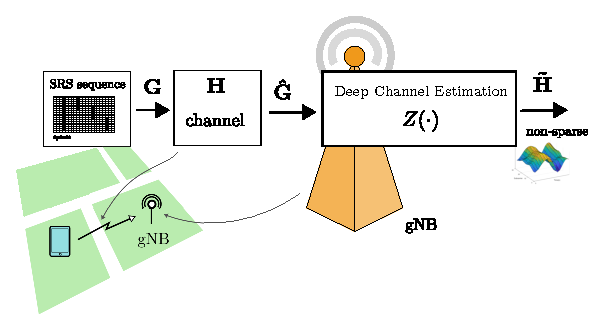
\includegraphics{chapters/part_uplink/figures/channel_estimation_approach_v2.eps}
    \caption{The Deep Channel Estimator is tasked with estimating the channel conditions $H$ from the received \gls{srs} sequence $\hat{G}$.}
    \label{fig:my_label}
\end{figure*}
We define $H[t]$ as the frequency response of the time-variant channel at time $t$. We furthermore define $G[t]$ as a generated and transmitted \gls{srs} sequence for some bandwidth $W$ and with some configuration $C$. Bold $\mathbf{H}$ and $\mathbf{G}$ denotes the sequence of past $m$ samples; e.g. $\mathbf{H} = H[t],H[t-1],...,H[t-m]$.

\begin{equation}\label{eq:channel_est_input}
    \mathbf{\hat{G}} = \mathbf{G} \mathbf{H}
\end{equation}

The received and demodulated \gls{srs} sequence $\mathbf{\hat{G}}$ is denoted by Eq. (\ref{eq:channel_est_input}) where the operation is seen as a multiplication, thus $\mathbf{\hat{G}}$ is in the frequency domain over the used subcarriers denoted by $W$.

\begin{equation}\label{eq:data_imputation}
    \mathbf{\widetilde{H}} =   \mathbf{Z}(\mathbf{\hat{G}},W_Z, \theta_Z)
\end{equation}


Due to the configuration of $\mathbf{G}$, $\mathbf{\hat{G}}$ is sparse and thus not a full approximation of the channel over the bandwidth. We seek to learn a mapping function $\mathbf{Z}$ that maps between $\mathbf{\hat{G}}$ and the full frequency response of the channel denoted $\mathbf{\tilde{H}}$ as described by Eq. (\ref{eq:data_imputation}), this we also term \emph{data imputation} due to the sparsity of the input data.


\begin{equation}\label{eq:loss_function_channel_est}
    W_Z, \theta_Z = {arg\,min} \frac{1}{T}\sum_t || \mathbf{\widetilde{H}} - \mathbf{H}|| ^2
\end{equation}

We seek to obtain the best set of weights, $W_Z$ that minimizes the mean squared error between the sparse \gls{srs} sequence and the actual frequency response of the channel. To do this, we construct a deep convolutional neural network. The intuition behind the architecture is to compress the sparse sequence and extract relevant information from it. A decompressor type output structure is then tasked with learning the right "reconstruction" from a latent and compressed layer. This model structure is similar to the hour-glass structure as used in state-of-the-art image processing models such as \cite{DeepPrior}. 

\subsection{Data foundation}
The problem is formalized as a supervised problem where the channel conditions are the target values. The objective of the deep learning model is then to approximate the channel matrix $H$ using a sparse and noisy received \gls{srs} sequence $\hat{G}$. An example of a transmitted \gls{srs} sequence and the resulting received \gls{srs} sequence can be seen in Fig. \ref{fig:srs_sequence_example}. 

\begin{figure*}
    \centering
    \subfloat[Transmitted \gls{srs} sequence]{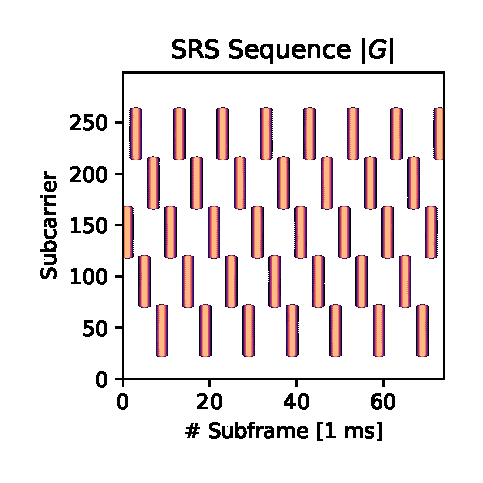
\includegraphics[width=0.33\textwidth]{chapters/part_uplink/figures/G.eps}}
    \subfloat[Channel conditions]{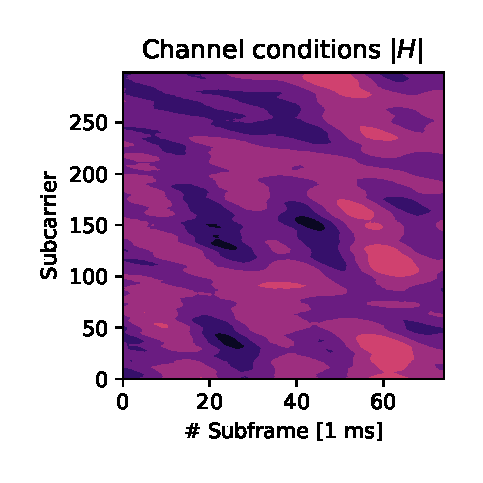
\includegraphics[width=0.33\textwidth]{chapters/part_uplink/figures/H.eps}}
    \subfloat[Received \gls{srs} sequence]{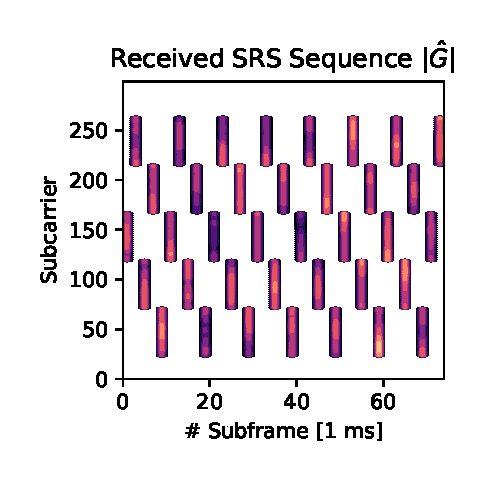
\includegraphics[width=0.33\textwidth]{chapters/part_uplink/figures/G_hat.eps}}
    \vspace{2em}
    \caption{The \gls{srs} sequence essentially serves as a \emph{mask} for the channel conditions resulting in a sparse matrix of received channel coefficients.}
    \label{fig:srs_sequence_example}
\end{figure*}

A set of channel conditions are emulated using the \gls{tdl} model as specified by $3$GPP and ITU \cite{3GPP38901, ITU2412} and as described in Section \ref{sec:stochastic_channel_model}. The implementation of both the channel model and the \gls{srs} sequence is detailed in Section \ref{ch:monster}. The \gls{srs} sequence is generated using several parameters, some related to bandwidth, some related to the periodicity. A brief introduction can be found in Section \ref{sec:srs_sequence_definition}. A set of channel conditions and \gls{srs} sequences are simulated. The specific parameters can be found in Table \ref{tab:sim_param_channel_est}. Several parameters are noted in terms of vectors. The vectors note that the training dataset is composed of several varieties of both periods, and \gls{srs} sequences. More specifically, the dataset is composed of the configurations as depicted in Fig. \ref{fig:data_channel_estimation}. For a total of $6000$ \gls{lte} frames, the channel conditions were emulated using the \gls{tdl} model. Two separate datasets were emulated with different seeds but the same characteristics, composing a test and training set. 

\begin{figure}
    \centering
    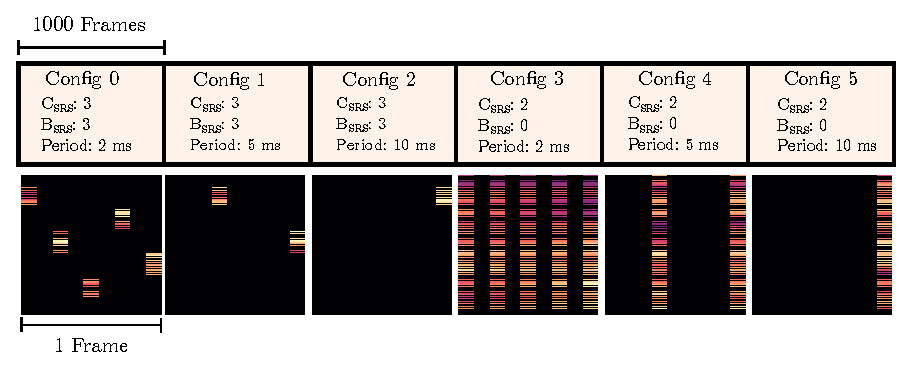
\includegraphics{chapters/part_uplink/figures/data_channel_estimation.eps}
    \caption{A variety of \gls{srs} sequences are produced with different configurations. A single frame from each configuration is visualized in the bottom row. }
    \label{fig:data_channel_estimation}
\end{figure}



\begin{table}[]
\centering
\begin{tabular}{l|l}
\toprule
\textbf{Parameter}                 & \textbf{Value} \\ \midrule
$f_c$ & $6$ GHz \\
NULRB         & $25$             \\
$C_{SRS}$   &  $[2,3]$               \\
$B_{SRS}$ & $[0,3]$ \\
Period & $[2, 5, 10]$ ms \\
\# Frames per config & $1000$ \\
\# Total frames & $6000$ \\
Delay spread  & $300e-9$         \\
Delay profile & TDL-E          \\
% Doppler Shift & $D_S = \frac{f_c v}{c}$ \\
% Coherence time & $T_D = \frac{1}{4D_S}$ \\
% Coherence bandwidth & $\frac{1}{2T_D}$ \\
% \# Frames & 2000 \\
User velocity & 5 m/s         
\end{tabular}
\vspace{1em}
\caption{Simulation parameters used for data set generation.}
\label{tab:sim_param_channel_est}
\end{table}

\subsection{Model Architecture}
The model architecture can be described as an hour-glass type Deep Learning model, as usually seen used in auto-encoders \cite{Nielsen2015}. The model architecture is visualized in Fig. \ref{fig:model_architecture_channel_estimation}. In brief terms the model is tasked with observing sparse and noisy \gls{srs} sequence and through a set of dimensionality reducing layers it obtains a latent layer, $\mathcal{L}$, which is tasked with learning the most important characteristics of the channel. A set of up-scaling layers are then applied to scale from the reduced dimension of the latent layer $\mathcal{L}$ to the original dimensions of the resource grid. Doing so enables for optimization using the loss function seen in Eq. (\ref{eq:loss_function_channel_est}) utilizing the true channel coefficients $\mathbf{H}$ and the estimated channel coefficients $\mathbf{\widetilde{H}}$. Moreover, the model makes use of so-called residual connections. The use of residual connections have shown to be effective in image recognition problems, as the information bottleneck imposed by the dimensionality reduction layers restricts learning and the \emph{knowledge} passed through the sequential layers of the model \cite{He2016DeepRecognition}. In simple terms, the symmetrical properties of the hour-glass type model allow for connections between the input and the output layers. 

\begin{figure*}
    \centering
    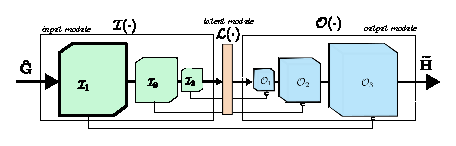
\includegraphics{chapters/part_uplink/figures/model_architecture.eps}
    \caption{Model architecture for Deep Learning based channel estimation utilizing an hour-glass structure with residual connections.}
    \label{fig:model_architecture_channel_estimation}
\end{figure*}

A set of standard components for building deep learning models are utilized in this model architecture. A brief overview of the layers and their respective definitions can be found in Section \ref{ch:mlbasics}. For this particular model, the model can be split into 3 separate parts, we term these the \emph{input, latent and output} modules, and define them as $\mathcal{I}(\cdot), \mathcal{L}(\cdot), \mathcal{O}(\cdot)$ respectively. Thus the model $Z(\cdot)$ is composed of three sub-modules, i.e. 

\begin{equation}
    Z(\mathbf{\hat{G}}) = \mathcal{O}\{\mathcal{L}[\mathcal{I}(\mathbf{\hat{G}})]\}
\end{equation}

\paragraph{Input module}
The input module, $\mathcal{I}(\cdot)$, is tasked with applying a set of image processing operations to the matrix $\mathbf{\hat{G}}$. These can furthermore be specified (in sequence) as:

\begin{enumerate}
    \item $2$D Convolution
    \item \gls{relu} activation function
    \item Batch Normalization
    \item Max Pooling
\end{enumerate}

We term this sequence a single \emph{layer} in the input module. The input module consists of a total of $3$ layers, and each utilizes the above set of modules.

\paragraph{Latent module}
The latent module, $\mathcal{L}(\cdot)$, is tasked with conveying the reduced information of the observed \gls{srs} sequence from the \textit{input module} to a set of fully connected and adaptive weights. For this module only a single layer is considered. The layer consists of the following sequence
\begin{enumerate}
    \item Fully-connected dense layer
    \item \gls{relu} activation function
    \item Drop-out
\end{enumerate}

\paragraph{Output module}
The output module, $\mathcal{O}(\cdot)$, is tasked with interpreting the reduced information of the latent layer and produce an image that is the same size as the input image. Using a sequence of interpolation and up-sampling filters, this can be accomplished. Specifically, a single layer of the output module is the output of the sequence below:

\begin{enumerate}
    \item Upsampling
    \item 2D Interpolation
    \item \gls{relu} activation function
    \item Batch Normalization
\end{enumerate}


\paragraph{Residual connections}
Each of the input and output modules consists of 3 \emph{layers}. A connection between the layers is added. If $\mathcal{I}(\cdot)_3$ denotes the output of the final layer in the input module, a connection is added to the first layer of the output module as follows $\mathcal{O}(\cdot)_{1}^{'} = \mathcal{I}(\cdot)_3  + \mathcal{O}(\cdot)_1$. In order to establish such a connection, the size of the tensors must be the same size. The residual connections are visualized in Fig. \ref{fig:model_architecture_channel_estimation} for each of the input and output layers and has shown during training to improve performance with $50-70\%$.

\paragraph{Implementation}
The full implementation of the model can be found in \cite{Thrane2020RepositoryLearning}.


\paragraph{Hyperparameters}
A grid search was utilized to discover the best performing hyper-parameters. The parameters for the convolutional layers can be seen in Table \ref{tab:channel_estimation_hyperparameters_conv}. The remainder of the hyper-parameters can be seen in Table. \ref{tab:channel_estimation_hyperparameters}


\begin{table*}[]
\begin{tabular}{@{}lllllll@{}}
\toprule
Layer/Parameter & Kernel Size & Padding & Stride & Filters & Leaky ReLU & Max Pooling \\ \midrule
$\mathcal{I}_1$            & (9,9)       & 4       & 1      & 10      & 0.2        & (2,2)       \\
$\mathcal{I}_2$              & (1,1)       & 0       & 1      & 10      & 0.1        & (2,2)       \\
$\mathcal{I}_3$            & (5,5)       & 2       & 1      & 1       & 0.2        & (2,2)       \\
$\mathcal{L}_1$              & -           & -       & -      & -      & -          & -           \\
$\mathcal{O}_1$              & -           & -       & -      & 1       & ReLU       & -           \\
$\mathcal{O}_2$               & -           & -       & -      & 10      & ReLU       & -           \\
$\mathcal{O}_3$               & -           & -       & -      & 10      & ReLU       & -           \\ \bottomrule
\end{tabular}
\vspace{2em}
\caption{Parameters of the convolutional layers used in the model. The layers of the output module interpolate the tensors to the size of the corresponding input module layer.}\label{tab:channel_estimation_hyperparameters_conv}
\end{table*}

\begin{margintable}
\begin{tabular}{@{}ll@{}}
Parameter     & Value  \\ \midrule
Learning Rate & $0.001$  \\
Drop-out      & $0.05$   \\
Weight Decay  & $0.0001$ \\
M             & $75$     \\
Batch size    & $60$    \\ \bottomrule
\end{tabular}
\caption{Hyper-parameters for the deep channel estimation model.}\label{tab:channel_estimation_hyperparameters}
\end{margintable}

% \paragraph{Data augmentation}
% The different \gls{srs} sequences utilized offer a limited dataset. Upon inspection of training it was observed that by increasing the number of differences in observation improved generalization. More specifically, this was completed by introducing 2 strategies for augmenting the data. A set of so-called masks were applied. This procedure was only enabled due to the availability of the true channel conditions over all resource elements.

% \begin{itemize}
%     \item Random sampling of points from the channel conditions, limited by the original length of the \gls{srs} sequence
%     \item Random adjustment of the position of the \gls{srs} sequence in frequency. E.g. adjusting the starting frequency position randomly.
% \end{itemize}

% The results of utilizing such data augmentation are described below.

\subsection{Results}
The convergence result of the training can be seen in Fig. \ref{fig:training_test_error_channel_estimator}. The performance during testing is lower than training due to the use of dropout layers. These layers are not enabled during testing (unless Bayesian approximation is applied) to ensure the best generalisation, and thus the best performance of the model is achieved when testing. A learning rate scheduler was applied, meaning an early stopped was executed when the learning rate dropped below a certain magnitude (See \ref{subsec:lr_scheduler}).
\begin{figure}
    \centering
    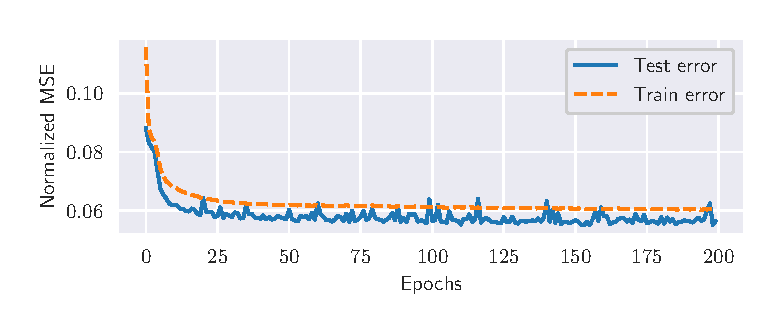
\includegraphics{chapters/part_uplink/figures/results/channel_estimation/Training_test_error.eps}
    \caption{The \gls{mse} of the model during training and evaluated on the test set each \emph{epoch}}
    \label{fig:training_test_error_channel_estimator}
\end{figure}

The model is evaluated for each \gls{srs} configuration as visualized in Fig. \ref{fig:data_channel_estimation}. The results in terms of normalized \gls{mse} can be observed in Fig. \ref{fig:srs_configuration_error_boxplot} for all used configurations. Two common interpolation methods are added for comparison, more specifically, a linear estimator, and a spline estimator (degree $3$) \cite{2020SciPy-NMeth}.  For the sparse \gls{srs} sequences, where frequency hopping is in full effect, the proposed method outperforms regular interpolaters significantly. For instance, for \emph{config $3$} the regular estimators performs poorly when faced with the sparse nature of the configuration. The performance of the spline estimator for \emph{config $3$} is on average at $1.5$ which is not visualised on the plot due to the magnitude in difference. The performance of the proposed method decrease as the period of the \gls{srs} sequence is increased as noted by \emph{config 0, 1} and \emph{2}. This is also the case for \emph{config $3$, $4$} and $5$ but to a much less degree. In any case the proposed method outperforms common channel estimation functions by, in the best case (\emph{config $3$}) by a factor of $19$, and in the worst case a factor of $5$ (\emph{config $0$}).
\begin{figure*}
    \centering
    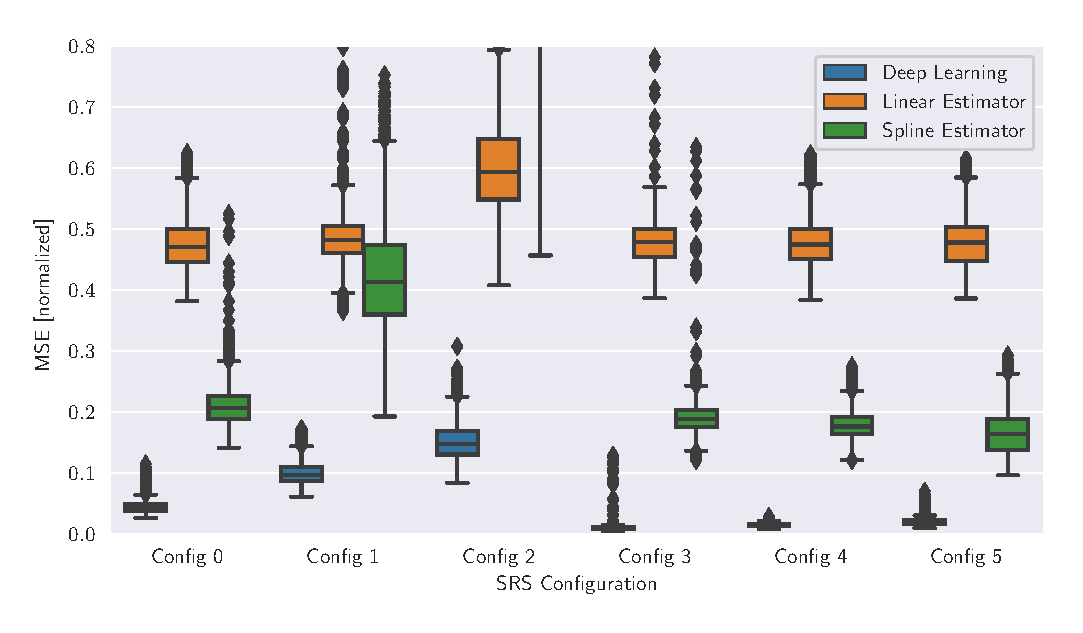
\includegraphics{chapters/part_uplink/figures/results/channel_estimation/srs_configuration_error_boxplot.eps}
    \caption{Evaluation of the proposed method compared to common channel estimators for different configurations of \gls{srs} sequence. (Lower is better)}
    \label{fig:srs_configuration_error_boxplot}
\end{figure*}

Examples of predictions for all the different configurations can be observed in Fig. \ref{fig:prediction_example_grid}. The estimated channel $\mathbf{\widetilde{H}}$ is seen along with the true channel conditions.
\begin{figure}
    \centering
    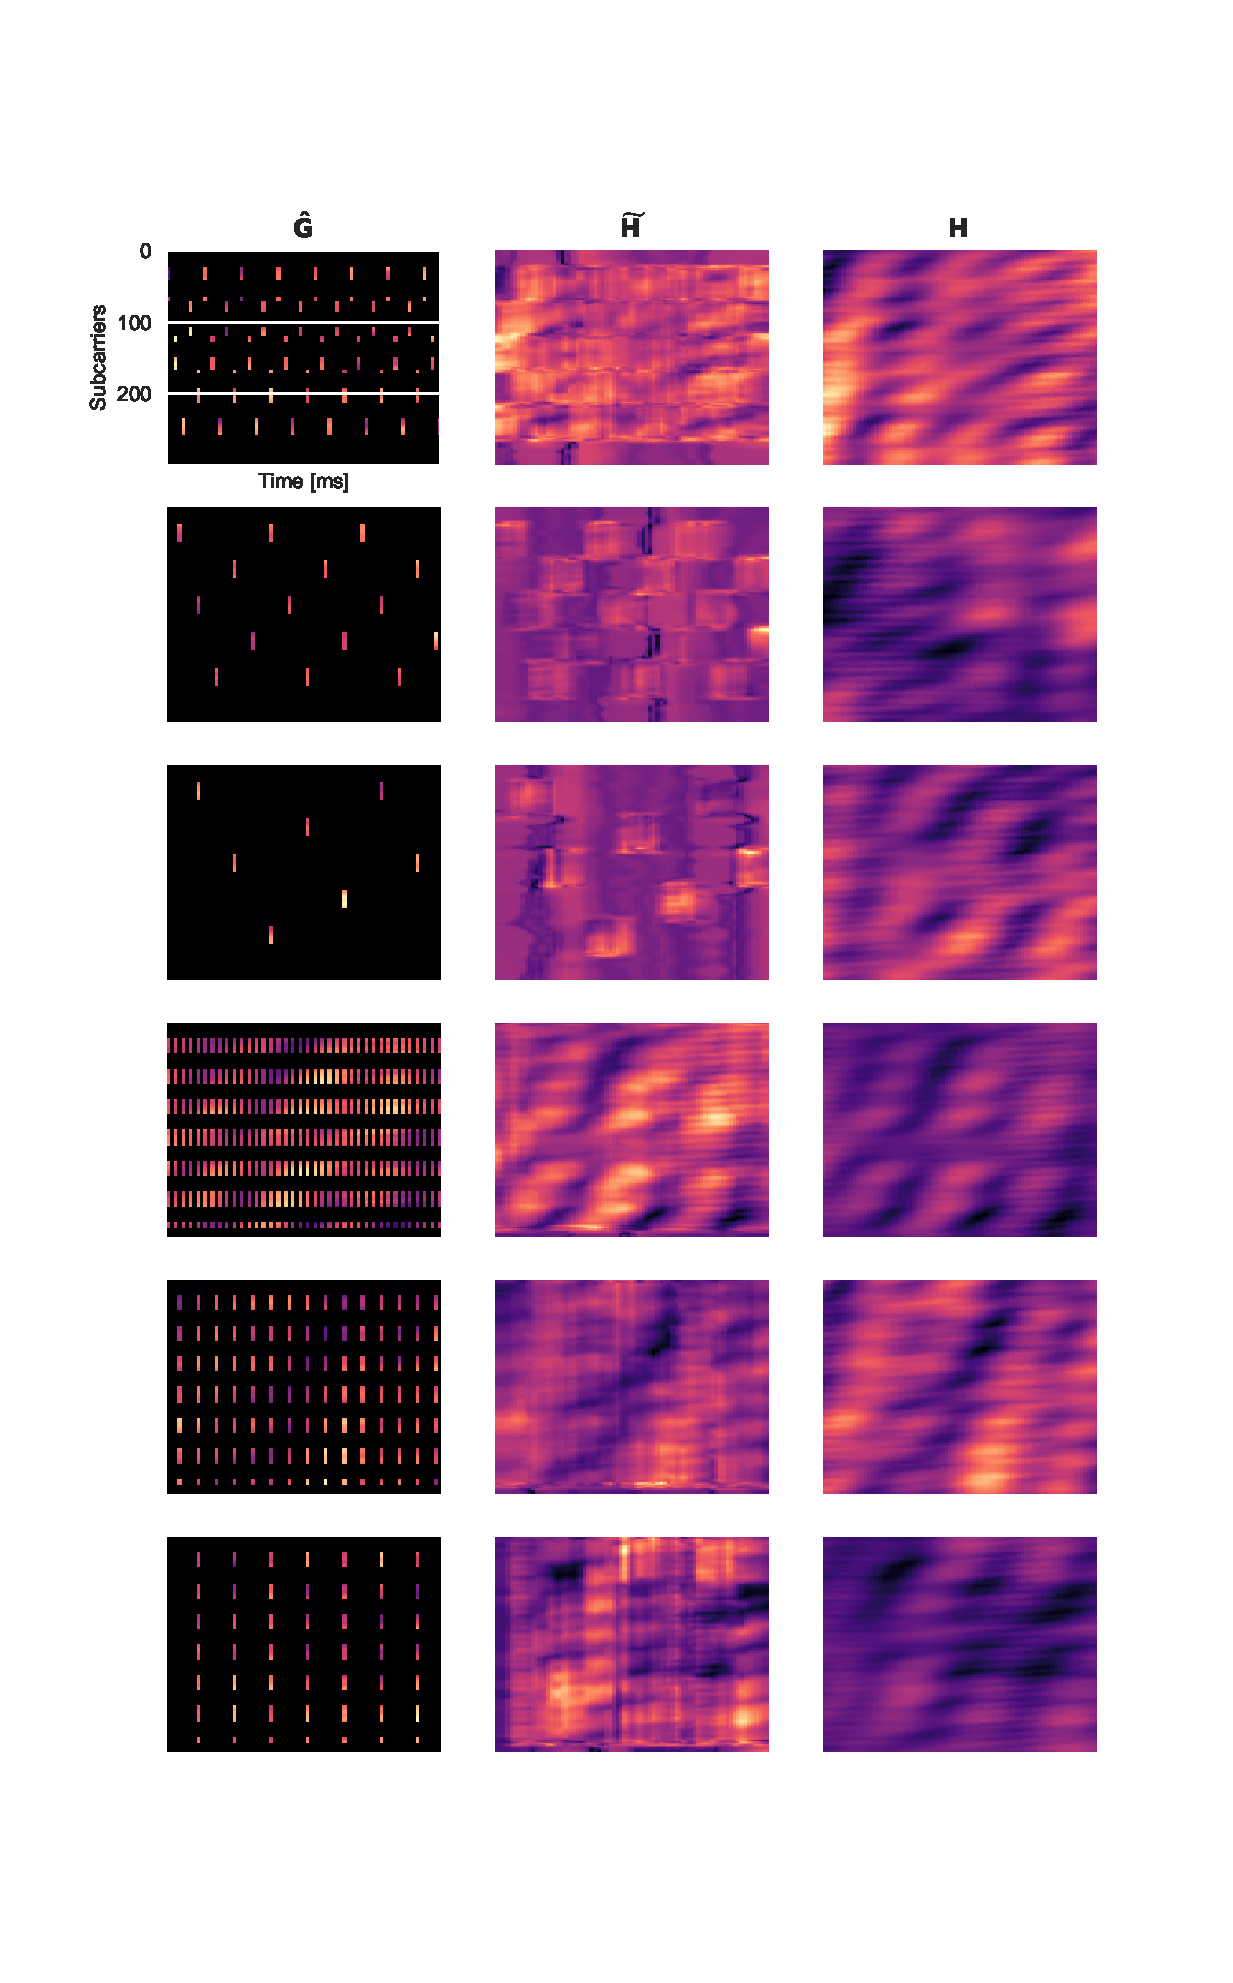
\includegraphics[width=1.1\textwidth]{chapters/part_uplink/figures/results/channel_estimation/prediction_example_grid.eps}
    \caption{Prediction examples of the proposed method.}
    \label{fig:prediction_example_grid}
\end{figure}

\subsection{Discussion}
The proposed method for channel estimation is trained at a set of fundamental channel characteristics. These channel characteristic are formalised using a set of simulation parameters, such as user velocity and the carrier frequency. The resulting coherence time and bandwidth of these parameters are considered the fundamental characteristics of the channel. From the visual examples of the predictions, some sense of the coherence time can be observed. For the given simulation parameters, the resulting coherence time is \textcolor{red}{XX} ms, which can be visually inspected from both the true channel conditions and the estimated channel conditions in Fig. \ref{fig:prediction_example_grid}. For instance, the predicted channel conditions of row 1 (\emph{config $0$}) a change in channel magnitude is observed 4-5 times which approximates the number of coherence blocks within the time frame visualised. However, a key issue of training arises. If the proposed method is capable of fundamentally deconstructing the channel conditions from a sparse set of measurements, how well would it be able to deconstruct a sparse set of measurements with inherently different channel characteristics? Furthermore, how often would the training be required? Unfortunately, such questions are difficult to answer without doing additional experiments and evaluations. A solution to this is presented in Section \ref{sec:research_trends_channel_estimation}.

The method performs well for sparse \gls{srs} sequences, as seen by the performance of \emph{config} $0$ to $2$. A decrease in channel estimation performance is observed with an increase in the periodicity of the \gls{srs} sequence.  A decrease in performance is also the case in \emph{config} $3$ to $5$, but with significantly lower magnitude. The result shows that channel estimation performance is determined by the periodicity and bandwidth of the \gls{srs} sequence. It is shown that the proposed method outperforms traditional channel estimation functions such as the spline or the linear channel estimator. Traditional approaches of channel estimation require tricks of the trade to reduce and remove values of overfitting or extrapolation where no \gls{srs} sequence is available - this is not the case for the proposed \gls{dl}-based channel estimator.

Ultimately, improving channel estimation reduces the amount of sub-optimal transmission configurations. For instance, in a channel-aware scheduler, individual multi-path fading components are utilised to improve the \gls{sinr} of a specific set of \glspl{ue}. Having inaccurate or incomplete channel estimation would mean sub-optimal decisions in choosing such resources for scheduling and thus a reduced data rate. The current results are presented for a \gls{siso} transmission case and remain untested for a \gls{mimo} transmission case. The high dimensionality of \gls{mimo} pilot signals are inherently and fundamentally suitable for the further development and application of \gls{dl}-based channel estimators but remain to be tested. 

\subsection{Conclusion}
A channel estimator for \gls{srs} pilot sequences of different configurations has been presented. The proposed method utilises image processing capabilities from the extensive toolbox of Deep Learning to learn from the sparse samples provided by such pilots configurations in a supervised fashion. The results show that the proposed method is capable of improving channel estimation performance significantly compared to traditional channel estimators such as linear and spline, in a \gls{siso} uplink transmission case. The channel estimation performance is enhanced by up to a factor of $19$ compared to traditional methods. In conclusion, Deep Learning utilising image processing techniques is a suited interpolator that can be applied to channel estimation in \gls{lte} and \gls{nr} uplink transmission.

\section{Uncertainty measure}
Given the learning capabilities of the deep channel estimator, and the above presented achievable performance. It was perceived that the proposed approach is capable of generalizing channel characteristics given a wide range of sparse \gls{srs} sequences. If such is the case, and the model is well-tuned, it is expected that future channel characteristics can be inferred given the past experiences. It is therefore desired to explore such an application, where the learned model is also capable of providing an intelligent decision regarding the most optimal placement of the future \gls{srs} sequence. In order to do so, the idea of utilizing Bayesian Approximation seemed appropriate (as described in \ref{ch:mlbasics}), since dropout layers are utilized in the model structure. The model can be \gls{mc} sampled to obtain an approximation of the posterior distribution. Taking action for optimized placement can then be formalized as the corresponding sequence of necessary initial steps:

\begin{enumerate}
    \item Initialize an empty resource grid, place an initial pilot sequence randomly.
    \item Apply channel model.
    \item Sample the learned model with the sparse resource grid to obtain a posterior distribution of the entire resource grid.
    \item Average over I and Q components for all \gls{ofdm} symbols.
    \item Obtain the standard deviation over the entire resource grid.
    \item Find the sequence of subcarriers across the entire frame with the highest standard deviation.
\end{enumerate}

The subcarriers with the highest standard deviation are a set of subcarriers where the learned channel estimator is most uncertain in the predictions. The hypothesis is that by utilizing this information, the next pilot sequence can then be placed in a position that would improve channel estimation predictions. Step 2-5 are then repeated for any future subframes where a pilot placement is to be predicted. The number of samples required in step 2 is directly related to the accuracy of the posterior distribution approximation, given that the model represents a good approximation of the underlying function. For this particular set of results, the network is sampled $100$ times. Correctly, step 5 is completed by averaging the standard deviation over all \gls{ofdm} symbols for the entire frame. The subcarriers that have the highest standard deviation is then identified. The future \gls{srs} sequence is placed such that $N/2$ samples of the pilot bandwidth is distributed on either side of the subcarrier with maximum standard deviation. The results for utilizing the uncertainty metric for a pilot placement strategy can be found below. 

An example of the placement procedure can be found in Fig. \ref{fig:decision_example} for a fixed periodicity. The cold start of the algorithm is presented,  showing the first sequence is placed at random. The maximum standard deviation is used for placing the next \gls{srs} sequence, which in turn lowers the channel estimation error. The first two  \gls{srs} sequences are presented, along with the last two throughout $75$ ms for $300$ subcarriers. 

\begin{figure}
    \centering
    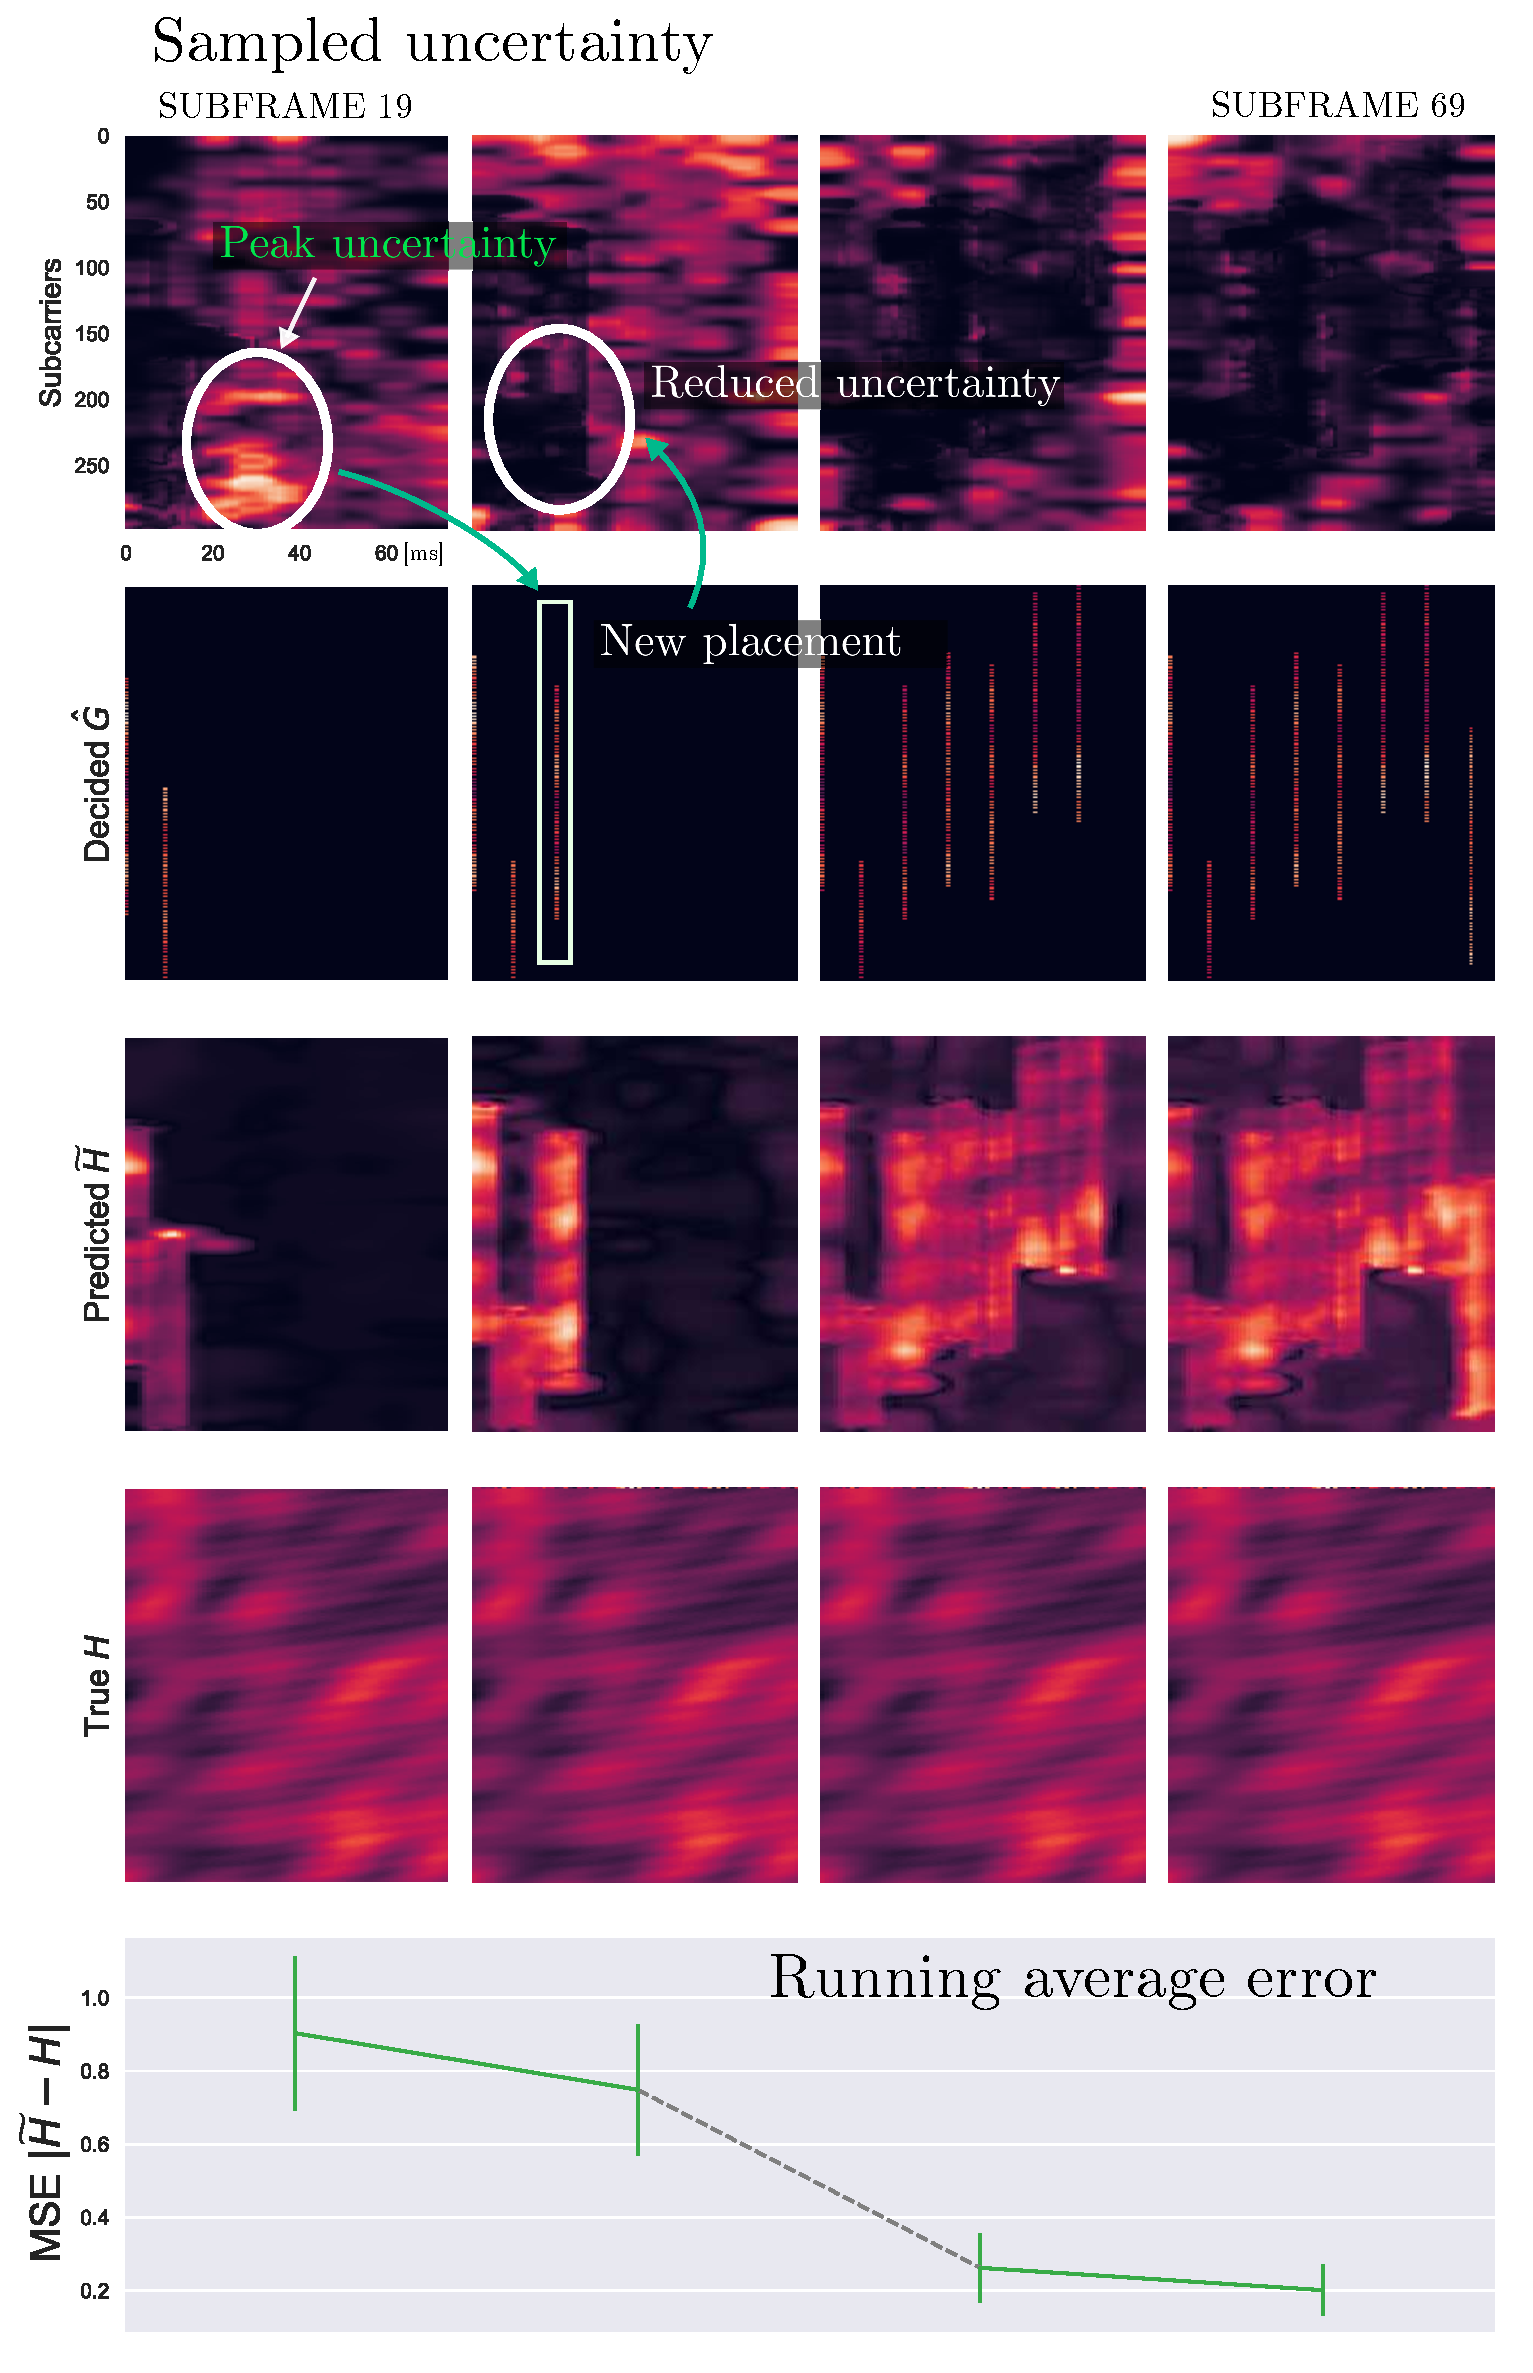
\includegraphics{chapters/part_uplink/figures/results/channel_estimation/decision_example_imshow.eps}
    \caption{The initial decisions of pilot placement achieved by sampling the uncertainty metric of the \gls{dnn}.}
    \label{fig:decision_example}
\end{figure}

\subsection{Results}
To evaluate the strategy of the uncertainty, the length of the  \gls{srs} sequence is varied. The length is described in terms of overhead (\%). Overhead is the percentage of all available resource elements versus resource elements over an entire frame used for the \gls{srs} sequence. The results can be seen in Fig. \ref{fig:overhead_channel_estimation} (lower is better). Three schemes for pilot placement are compared to the proposed method. 

1) A random scheme where a \gls{srs} sequence with a defined length (determined by the overhead percentage) is placed at random throughout the frame. 

2) The actual \gls{srs} sequence with enabled frequency hopping noted by the standard (see section \ref{sec:srs_sequence_definition}). Examples of this can be seen in Fig. \ref{fig:prediction_example_grid}. 

3) The utilized uncertainty metric for placing the next set of pilots.

It can be seen that placing pilots randomly for up to $3\%$ of overhead outperforms both schemes for placing the \gls{srs} sequence. The utilized \gls{srs} sequence offers improved channel estimation performance than the use of the uncertainty metric for up to $3\%$ of overhead. After which both the proposed method and the \gls{srs} sequence outperform placing pilots randomly. A linear increase in channel estimation performance is observed with an increase in overhead. The proposed method outperforms the use of regular \gls{srs} sequences with $2-17\%$ from $3-9\%$ overhead, respectively.

\begin{figure}
    \centering
    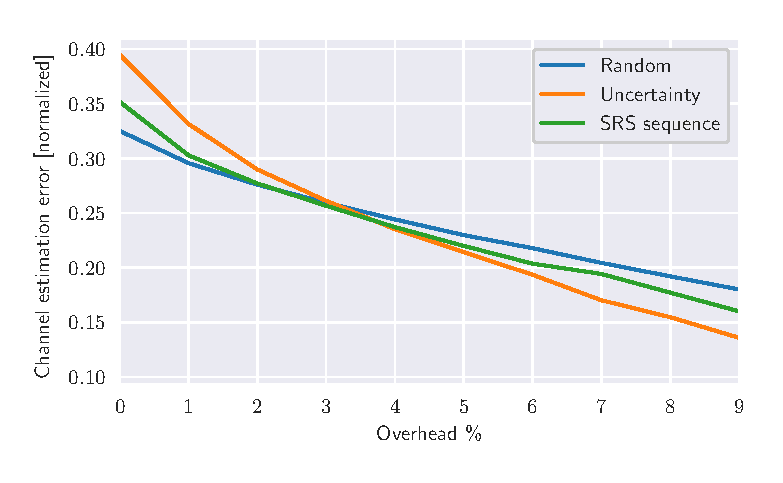
\includegraphics{chapters/part_uplink/figures/results/channel_estimation/overhead_comparison_scheme.eps}
    \caption{Channel estimation performance of different \gls{srs} placement schemes}
    \label{fig:overhead_channel_estimation}
\end{figure}


\subsection{Discussion}
A decrease in channel estimation performance at lower percentage of overhead ($0$ to $3\%$) is observed for the proposed method of \gls{srs} placement compared to that of non-channel-aware pilot placement schemes. This amount of overhead effectively reduces the bandwidth of the \gls{srs} sequence resulting in a sparsity increase. As was observed for the deep channel estimator the increase in sparsity, not only in time but also in frequency, decreases the resulting channel estimation error. More specifically, the overhead of $3\%$ accumulates to a bandwidth of \textcolor{red}{XX} subcarriers. So, the decrease in channel estimation error is related to the pilot sparsity - this indicates that the learned channel estimation function, at sparse \gls{srs} sequences, does not represent the underlying function of the channel. So, if the available pilot symbols are reduced, the \gls{csi} available for learning is also reduced. In short, the performance decrease at lower overhead percentages show the key issue of the proposed method; training examples.

The deep channel estimator is trained in a supervised fashion, meaning that the true channel coefficients are required to be known. The objective is to learn a function that is capable of mapping from a sparse pilot sequence to the channel coefficients over the entire \gls{ofdm} resource grid. In practice, such data sets could be generated by utilizing a collection of masks and data augmentation techniques on full bandwidth pilot sequences for every coherence block. For \glspl{ue} moving at high velocity, this approach may result in unfeasible training routines as the coherence block would likely be faster than the expected computational time required for updating the weights.

To effectively provide a reasonable approximation of the posterior distribution, the model is required to be sampled a sufficient number of times. Increasing the number of samples increases the accuracy of the posterior distribution approximation, however at the cost of increased computational runtimes. The proposed method for \gls{srs} sequence placement, provides with improved channel estimation results compared to non-channel-aware schemes for more than $3\%$ of overhead. However, the method suffers from extensive computational complexity when \gls{mc} sampling the network. For this method to be feasible for practical systems, a significant number of challenges have been identified (See section \ref{sec:channel_estimation_challenges}). 

\subsection{Conclusion}
A pilot placement method for improving channel estimation performance have been proposed using Bayesian approximation techniques on a learned deep channel estimator function. The learned deep channel estimator is sampled to offer an approximation of the posterior distribution over the entire resource grid, which is used to infer the best position of future pilot sequences. The proposed method is capable of outperforming standardized \gls{srs} sequences, and random placements when the sparsity of the pilot sequence is reduced to at least $3\%$ of overhead with up to $17\%$. Significant challenges in terms of runtime and computational complexity have been identified for use in practical \gls{lte} and \gls{nr} systems. Finally, it has been shown that increased optimization of channel estimation can be achieved by strategically placing future pilots to exploit the statistics of the channel learned through the \gls{dnn} structures.

\section{Deep prior channel estimation}\label{sec:research_trends_channel_estimation}
A key challenge of the proposed method can be narrowed down to the practicalities of training. It is unknown based on the current results how it performs for differences in channel characteristics, but nonetheless, the data set for training the model needs to be generated. The authors in \cite{Balevi2019} propose a solution for this. A state-of-the-art image algorithm known as \emph{Deep Image Prior} is applied on \gls{mimo} channel estimation for \gls{lte} cellular systems. \emph{Deep Image Prior} is a method published in \cite{DeepPrior} that utilize a search for an optimum solution in the space of neural network parameters. A method like the one developed in this dissertation seek to minimize an objective function (sum-of-squares) with a search in the input space. \emph{Deep Image Prior}, on the other hand, seeks to find the set of neural network parameters that offer the best prediction. Unlike the proposed model, this is not done by searching in input space, but rather done searching in the space of the neural network parameters. The intuition is that the structure of the network can offer a \emph{strong} enough prior and by itself sufficiently capture the necessary statistics  - without requiring any training. The authors show that a convolutional neural network without any supervised training is capable of outperforming \gls{ls} channel estimation for varying levels of \gls{snr}. The authors report a reduction of needed pilots by $68\%$ in an \gls{lte} transmission case with a channel coherence time interval of $4.5$ ms.

Deep Learning for channel estimation is a valuable tool for exploiting the correlations in the resource grid of \gls{ofdm} symbols. The use of the convolutional layers, as reported by results in this dissertation, and by state-of-the-art published research is ideal for capturing the statistics for accurate channel estimations. Furthermore, with the dimensionality increase of \gls{mimo} systems, the scalability properties of the convolutional layers in the \gls{dnn} is favourable for maintaining low complexity channel estimators. It has been shown that by using \gls{dl}-based channel estimators, the needed number of pilots can effectively be reduced. Reducing the number of pilots is essential for solving future issues related to \emph{pilot contamination}. The overhead and coordination required for pilot signals in future \gls{mimo} system cause significant problems and has has been termed \emph{pilot contamination}. The core issues of \emph{pilot contamination} and solutions hereof is outlined in the next chapter (see Chapter \ref{ch:channel_q_learning}), along with the application of a Deep Reinforcement Learning algorithm based on the experiences documented in this chapter.

\section{Identified Challenges}\label{sec:channel_estimation_challenges}
In this chapter, the application of Deep Learning for channel estimation has been shown. Furthermore, a method for \gls{srs} sequence placement to improve future channel estimation have been presented. The challenges of utilizing \gls{dnn} for channel estimation have been discussed throughout this chapter. A summary of the most noticeable challenges associated with deep channel estimators can be found below
\begin{itemize}
    \item Obtaining a training set for a deep channel estimator.
    \item Deep channel estimators are contingent on coherence time.
    \item Pilot placement strategies using posterior approximation techniques with \gls{mc} sampling of \gls{dnn} is a computational challenge.
\end{itemize}

\section{Summary}
The resource grid of \gls{lte} and \gls{nr} systems spanning time and frequency components are well suited for deep learning methodologies and image processing techniques. The experiences and results obtained through this chapter have laid the foundation for the novel solution presented in  Chapter \ref{ch:channel_q_learning}. The outcome of the above research can be summarized as the following.

\begin{itemize}
    \item Convolutional layers are efficient in learning correlation present in OFDM resource grids using \gls{srs} sequences
    \item A deep channel estimator can significantly reduce the required pilot symbols for accurate channel estimation.
    \item Novel solutions for further optimizing channel estimation can be engineered via pilot placement techniques 
\end{itemize}